\begin{center}

\begin{tikzpicture}[font=\small,overlay,
mycirclex/.style={draw, circle, minimum size=1.0em, inner sep = 0.2mm}, 
mydiamond/.style={draw, diamond, minimum size=0.78em, inner sep = 0mm}, 
myrectang/.style={draw, rectangle, minimum size=0.60em, inner sep = 0mm}, 
>=stealth]

\def\cola{blue} 
\def\colb{orange}
\def\colc{mygreen}
\def\cold{purple} 
\def\cole{gray} 
\def\colf{cyan}
\def\colg{brown}


\def\len{1.8cm}

% G1
\begin{scope}[local bounding box=bbox, xshift=-6.4cm]
\path<1-> node[mycirclex] (v1) at (1.0 * \len, 0) {$s$};
\path<1-> node[mycirclex] (v2) at (2.0 * \len, 0) {$a$};
\path<1-> node[mycirclex] (v3) at (3.0 * \len, 0) {$b$};
\path<1-> node[mycirclex] (v4) at (4.0 * \len, 0) {$c$};
\path<1-> node[mycirclex] (v5) at (5.0 * \len, 0) {$d$};
\path<1-> node[mycirclex] (v6) at (6.0 * \len, 0) {$t$};

\path<1-> [draw, \colx, ->, line width=0.04cm] (v1) -- (v2);
\path<1-> [draw, \colx, ->, line width=0.04cm] (v2) -- (v3);
\path<1-> [draw, \colx, ->, line width=0.04cm] (v3) -- (v4);
\path<1-> [draw, \colx, ->, line width=0.04cm] (v4) -- (v5);
\path<1-> [draw, \colx, ->, line width=0.04cm] (v5) -- (v6);

\path<1-> [draw, \colx, ->, line width=0.04cm, bend left = 40] (v1) to (v3);
\path<1-> [draw, \colx, ->, line width=0.04cm, bend left = 40] (v3) to (v5);
\path<1-> [draw, \colx, ->, line width=0.04cm, bend left =-40] (v2) to (v5);
\path<1-> [draw, \colx, ->, line width=0.04cm, bend left =-40] (v4) to (v6);

\path<1-> node at (1.5 * \len, 0.2cm) {$4$};
\path<1-> node at (2.5 * \len, 0.2cm) {$1$};
\path<1-> node at (3.5 * \len, 0.2cm) {$5$};
\path<1-> node at (4.5 * \len, 0.2cm) {$4$};
\path<1-> node at (5.5 * \len, 0.2cm) {$9$};

\path<1-> node at (2.0 * \len, 1.0cm) {$6$};
\path<1-> node at (4.0 * \len, 1.0cm) {$2$};
\path<1-> node at (5.0 * \len,-1.0cm) {$1$};
\path<1-> node at (3.5 * \len,-1.3cm) {$3$};

\end{scope}
%\path<1-> [draw, rounded corners] ($(bbox.south west) - (0.00cm, 0.25cm)$) rectangle ($(bbox.north east) + (0.1cm, 0)$);
%\node at ($(bbox.south) - (0.00cm, 0.2cm)$) [label=below:{$G_2 - G_1 = \{c\}$}]{};


\end{tikzpicture}
\end{center}
